\documentclass[12pt,letterpaper,boxed]{hmcpset}
\usepackage[margin=1in,headheight=14pt]{geometry}
\usepackage{amsfonts, amsmath, amssymb, enumerate, fancyhdr, gensymb, lastpage, mathtools, parskip, graphicx}
\usepackage{xcolor, tikz-cd}
\newcommand{\wg}[1]{\textcolor{violet}{#1}}
\newcommand{\OO}{\mathcal O}
\newcommand{\Q}{\mathbb Q}
\newcommand{\R}{\mathbb R}
\newcommand{\C}{\mathcal C}
\newcommand{\Z}{\mathbb Z}
\newcommand{\abs}[1]{\left|#1\right|}
\newcommand{\im}{\text{im }}
\newcommand{\inv}{^{-1}}
\newcommand{\normal}{\unlhd} %% one can also use \trianglelelefteq
\usepackage[shortlabels]{enumitem}

% Numbering macros
\pagestyle{fancy}
\lhead{Will Gilroy}
\chead{Algs Homework \#}
\rhead{03 November 2021}
\lfoot{}
\cfoot{}
\rfoot{Page\ \thepage\ of\ \pageref{LastPage}}

\linespread{1.5}

\newcommand\blankpage{
    \thispagestyle{empty}
    \addtocounter{page}{-1}
    \newpage}
\renewcommand\footrulewidth{0.4pt}

\begin{document}

\problemlist{Algorithms HW } 

%------------------------- Problem 1 -----------------------

\begin{problem}
	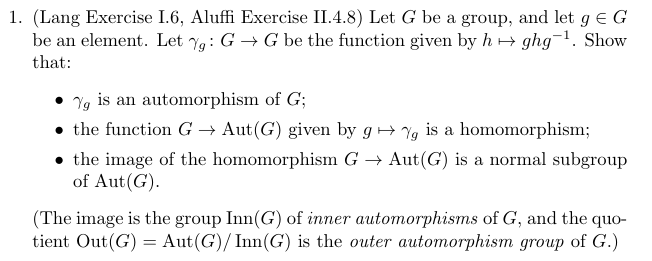
\includegraphics[scale=0.9]{1.png}
	\hfill
\end{problem}

\begin{solution}
\begin{enumerate}
	\item We show that $\gamma_g$ is a bijective homomorphism, for
	some fixed $g \in G$.
	Let $k, \ell \in G$ then we have \[
	\gamma_g(k \cdot \ell) = g \cdot
	(k \cdot \ell) \cdot g\inv = g \cdot k \cdot e \cdot \ell \cdot
	g\inv = (g \cdot k \cdot g\inv) \cdot (g \cdot \ell \cdot g\inv) =
	\gamma_g(k) \cdot \gamma_g(\ell),
	\]
	since group products are associative and by definition of the
	identity element. Hence $\gamma_g$ is a homomorphism for all $g
	\in G$.

	Now suppose $\gamma_g(h) = e$ for some $h \in G$ we have 
	\begin{align*}
		\gamma_g(h) &= e \\
		ghg\inv &= e \\
		(g\inv g)h(g\inv g) &= g\inv e g\\
		h &= g\inv e g \\ 
		h &= e.
	\end{align*} 
	Thus, $\gamma_g(h)$ is injective. Now let $k \in G$ and notice
	that $\gamma_g(g\inv k g) = g\cdot g\inv k g\inv g = k$. Moreover,
	$g\inv k g \in G$ since $G$ is closed under its group operation.
	That is, $\gamma_g$ is surjective for all $g \in G$.
	Hence, we have shown that $\gamma_g$ is an automorphism of $G$.

	\item Let $g,h \in G$.
	And let $f: G \to Aut(G)$ be the map $f(g)
	= \gamma_g$. 
	
	Consider the action of $\gamma_{gh}$ on
	some group element $k$. We have
	\begin{align*}
		\gamma_{gh}(k) &= (gh) k (gh)\inv \\
			&= (gh) k (h\inv g\inv) \\ 
			&= g (h k h\inv) g\inv \\
			&= (\gamma_g \circ \gamma_h)(k),
	\end{align*}
	holds for all $k \in G$. That is, we have shown $f(g \cdot h) = f(g)
	\circ f(h)$, where $\cdot$ denotes the product in $G$ and $\circ$
	denotes function composition --- the group operation in $Aut(G)$.
	Hence, $f$ is a homomorphism

	\item We show directly that $\im f$ is closed under conjugation by
	homomorphism in $Aut(G)$. Let $h \in Aut(G)$ and $\gamma_g \in \im
	f$. There then exists an
	inverse homomorphism $h\inv$ and consider the action of \[
		h \circ \gamma_g \circ h\inv.
	\]
	This is an automorphism since the composition of group
	homomorphisms is again a group homomorphism \wg{check this}.

	Let $k \in G$ and consider 
	\begin{align*}
		(h \circ \gamma_g \circ h\inv)(k) &= h(g \cdot h\inv(k) \cdot g\inv) \\
			&= h(g) \cdot k \cdot h(g\inv), && \text{since $h$ is a homomorphism}
	\end{align*}
	Moreover, $h(g) = g' \in G$ since $h$ is an automorphism of $G$.
	That is, we have shown $(h \circ \gamma_g \circ g\inv) = f(g') \in
	\im f$. And so, $\im f$ is a normal sunbgroup of $Aut(G)$ by
	definition.

\end{enumerate}
\end{solution}

\newpage

%------------------------- Problem 2 -----------------------

\begin{problem}
	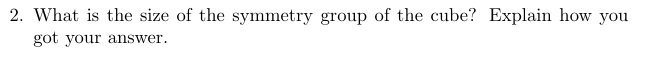
\includegraphics[scale=0.8]{2.png}
	\hfill
\end{problem}

\begin{solution}
\end{solution}

\newpage

%------------------------- Problem 3 -----------------------

\begin{problem}
	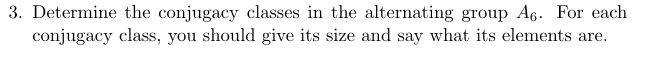
\includegraphics[scale=0.8]{3.png}
	\hfill
\end{problem}
\begin{solution}
We search for the conjugacy classes of $S_n$ whose elements are even
permutations. Note that this is a well-defined notion, since if
$\sigma, \tau \in S_n$ are even permutations then $\sigma \tau
\sigma\inv$ has a transposition decomposition whose length is a
product of three even numbers, and is thus even.

Recall that the conjugacy classes are exactly given by the type of a
permutation and that the number of valid conjugacy classes
correspond to the number of partitions of $n$. And so, we will
enumerate the partitions of $6$ and then acquire the conjugacy classes
of $A_6$ by choosing the classes which correspond to even partitions.
The partitions of $6$ are:
\begin{align*}
	\mathbf{[1,1,1,1,1,1,1]} &\qquad [2,2,2] \qquad \mathbf{[2,2,1,1]} \qquad [2,1,1,1,1]
	\qquad \mathbf{[3,3]} \qquad [3,2,1], \\ \qquad \mathbf{[3,1,1,1]}
	&\qquad \mathbf{[4,2]} \qquad [4,1,1] \qquad \mathbf{[5,1]} \qquad [6]. 
\end{align*}
The bolded types are those which correspond to even partitions and so
are the conjugacy classes of $A_6$. Recall that these are the types
whose number of entries have the same parity as $6$ (i.e. these are
the types with an even number of rows). Suppose $\sigma \in S_n$ has
type $[a_1, \cdots, a_k]$ then the parity of $\sigma$ is 
$(a_1 - 1) + \cdots (a_k -1)$, since each $a_i$ denotes the length of
a cycle which composes $\sigma$. Now notice 
$(a_1 -1) + \cdots (a_k -1) = \sum_i a_i - \sum_{i=1}^{k} (-1) = 6 -
2\ell = 6 - 2\ell$ is even. And so indeed the chosen permutations give
the conjugacy classes of $A_6$. 

However, we have a bit more counting to do. Recall that a conjugacy
$[\sigma] \subseteq S_n$ splits into two conjugacy classes in $A_n$
exactly when the type of $\sigma$ consists of distinct odd numbers,
and otherwise it splits into a single class in $A_n$. 
In our case we have $[3,3]$ and $[5,1]$ split into two clases in
$A_n$. Hence, overall we have $1 + 1 + 2 + 1 + 1 + 2 = 8$ conjugacy
classes in $A_6$. 

Next we determine the sizes of each conjugacy class in $A_6$. 
Note that the classes not of type $[3,3]$ and $[5,1]$ have the same
size as the corresponding classes in $S_n$. The classes of type
$[3,3]$ and $[5,1]$ split into two classes of equal sizes in $A_6$. 
Recall that the class type gives the sizes of the cycles in cycle
decomposition of $\sigma \in [\sigma]$. And so, we can determine the
size of each class by counting each distinct way of writing a
permutation with the given types.
For example, $[2,2,1,1]$ corresponds to $\sigma = (a_1,
a_2)(b_1b_2)(c_1)(d_1)$ where $a_i, b_i, c_i, d_i \in [n]$.
There are $6!$ ways to populate these numbers, but then we have
equivalent permutations given by cycling the elements in $(a_1,a_2)$
and $(b_1, b_2)$ and another equivalence given by interchanging the
cycles, then a final equivalence given by interchanging the two
trivial cycles. We do not need to consider any equivalence given by
interchanging the positions of the $2$-cycles and the trivial cycles,
since this was included in our enumeration of the partitions of $6$.
And so the number of elements in the class of type
$[2,2,1,1]$
is given by $\frac{6! = 720}{2 \cdot 2 \cdot 2 \cdot 2} = \frac{720}{16}$. 

A similar kind of counting gives us the following data. In the
following $\abs{[t_i]}$ means the number of elements in the
conjugacy class whose type is given by $[t_i]$.
\begin{align*}
	\abs{[1,1,1,1,1,1,1]} = 1 \qquad
	\abs{[2,2,1,1]} &= \frac{720}{16} \qquad
	\abs{[3,3]} = \frac{720}{3 \cdot 3 \cdot 2} \cdot \frac{1}{2} = \frac{720}{36} \qquad \\
	\abs{[3,1,1,1]} = \frac{720}{3 \cdot 3!} = \frac{720}{18} \qquad
	\abs{[4,2]} &= \frac{720}{4 \cdot 2} = \frac{720}{8} \qquad
	\abs{[5,1]} = \frac{720}{5} \cdot \frac{1}{2} = \frac{720}{10}
\end{align*}
Here the classes with type $[3,3]$ and $[5,1]$ in $S_n$ split into two
distinct equal sized classes in $A_6$ and so we have denoted the size
of each split class in the data above. Then we can write the class
formuala
\[
	1 + 45 + 2(20) + 40 + 90 + 2(72) = 360 = \abs{A_6}
\]
Showing that we have counted the size of our conjugacy classes
correctly.

Lastly, we write the elements of our classes. First consider the
classes which do not split in $A_6$. These classes have the same
elements in $A_6$ as they do in $S_6$. The type of the class tells us
the cycle decomposition of its elements. For example the class whose
type is $[2,2,1,1]$ contains even permutations whose cycle
decomposition is $\sigma = (a_1, a_2)(b_1, b_2)(c_1)(d_1)$ for $a_i,
b_i, c_i, d_i \in [n]$ and distinct. Since permutation type is
preserved by conjugation, this argument is well defined for a given
conjugacy class.
The same reasoning applies to the classes whose type is
$[1,1,1,1,1,1], [2,2,1,1], [3,1,1,1],$ or $[4,2]$.

The classes in $S_6$ whose type is $[3,3]$ or $[5,1]$ split into two distinct
equal size classes in $A_6$. 
\wg{how do we figure out which elements belong to which class?}



\end{solution}

\newpage

%------------------------- Problem 4 -----------------------

\begin{problem}
	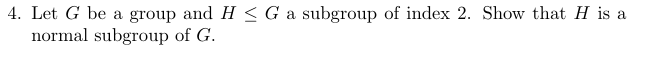
\includegraphics[scale=0.8]{4.png}
	\hfill
\end{problem}

\begin{solution}
Consider the action of conjugation on $H$ by some element $k \in G$.
If $k \in H$ then $k H k \inv = H$ since $H$ is a subgroup and thus is
closed under inversion and its group operation. And so, we
take $k \not \in H$.
Recall that $[H:G] = 2$ means that $G$ is partitioned into two cosets
of $H$, call them $H$ and $\overline H$.

Since $H$ is a subgroup of $G$ we have $e_G
\in H$ and so $k \in k H$. 
But then $e_G \in (kH)k\inv$ which implies $(kH)k\inv = H$ since
the cosets of $H$ partition $G$. This argument holds whether $kH = H$ or $kH =
\overline H$.
\wg{This seems, wrong, doesn't seem to depend on the fact that there's only two cosets}

We have shown that $k H k\inv = H$ for all $k \in G$, that is, $H$ is
normal in $G$.

\wg{Lang proves this using a lot of machinary of the orbits of group
actions and the kernel of group actions. That all seems more technical
than what I've done here, but not necessarily anymore slick. Is that
tru, or am I missing something?}

\end{solution}

\newpage


%------------------------- Problem 5 -----------------------

\begin{problem}
	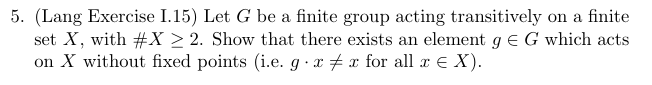
\includegraphics[scale=0.8]{5.png}
	\hfill
\end{problem}

\begin{solution}
\end{solution}

\newpage

%------------------------- Problem 6 -----------------------

\begin{problem}
	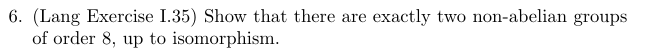
\includegraphics[scale=0.8]{6.png}
	\hfill
\end{problem}

\begin{solution}
\end{solution}

\newpage

%------------------------- Problem 7 -----------------------

\begin{problem}
	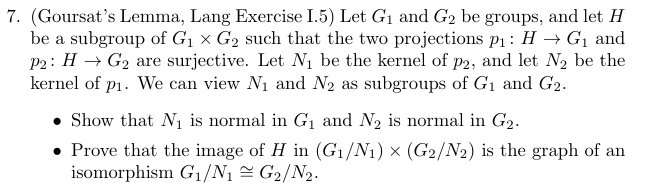
\includegraphics[scale=0.8]{7.png}
	\hfill
\end{problem}

\begin{solution}
\begin{itemize}
\item First, can view $N_i \leq G_i$ as say $p_1(N_1 = \ker p_2 =
\{(x,e_{G_2}) \in H\}) \leq
G_1$. This is indeed a subgroup of $G_1$ becuase if $x, y \in
p_1(N_1)$ then this means $(x, e), (y, e) \in N_2$ and so $(x +_{G_1} y, e)
\in N_2$ hence $x +_{G_1} y \in G_1$. And likewise for inverses and
the identity. Put another way, $p_1(N_1) \leq G_1$ since $N_1 \leq H$. 
Mutatis, mutandis for $N_2 \leq G_2$. 

Now we show that $N_1 \unlhd G_1$.
Let $x \in N_1 \leq G_1$ and let $g \in G_1$. Since $p_1: H \to G_1$
is surjective there exists $(g, y) \in H$ and $(g, y)\inv = (g\inv, y\inv) \in H$
since $H$ is a subgroup. Lastly $(x,e) \in H$ by definition of $\ker
p_2$. 
Now consider \[
	(g, y) \cdot_{G_1 \times G_2} (x, e) \cdot_{G_1 \times G_2} (g\inv, y\inv) 
	= (g x g\inv, e) \in H
\]
since $H$ is closed under $\cdot_{G_1 \times G_2}$. But then we have
shown $g x g\inv \in N_1 \leq G_1$. Thus, $N_1$ is closed under
conjugation and is normal in $G_1$. A very similar argument holds to
show that $N_2 \normal G_2$. 

\end{itemize}
\end{solution}

\newpage

\end{document}
